Los programas produjeron 220 mediciones de ordenamiento y 110 de
multiplicación. Todas pasaron la validación: los ordenamientos quedaron en
orden no decreciente y los algoritmos de un mismo problema entregaron la misma
suma de verificación.

\subsection{Ordenamiento}

La \cref{fig:sorting-scale} muestra un crecimiento compatible con
$O(n\log n)$ para los cuatro métodos. En $n=10^7$, \texttt{std::sort}
\cite{isocpp2024} fue el
más rápido con \SI{699.840}{\milli\second}; le siguieron Quick Sort con
\SI{938.731}{\milli\second}, Merge Sort con \SI{1114.274}{\milli\second} y
Patience Sort con \SI{2747.238}{\milli\second}. La memoria también separó las
estrategias: Quick Sort y \texttt{std::sort} alcanzaron cerca de
\SI{70.35}{\mebi\byte}, Merge Sort \SI{83.23}{\mebi\byte} por su arreglo auxiliar
y Patience Sort \SI{120.44}{\mebi\byte} por sus nodos y heap.

\begin{figure}[H]
    \centering
    \subfloat[Tiempo mediano.]{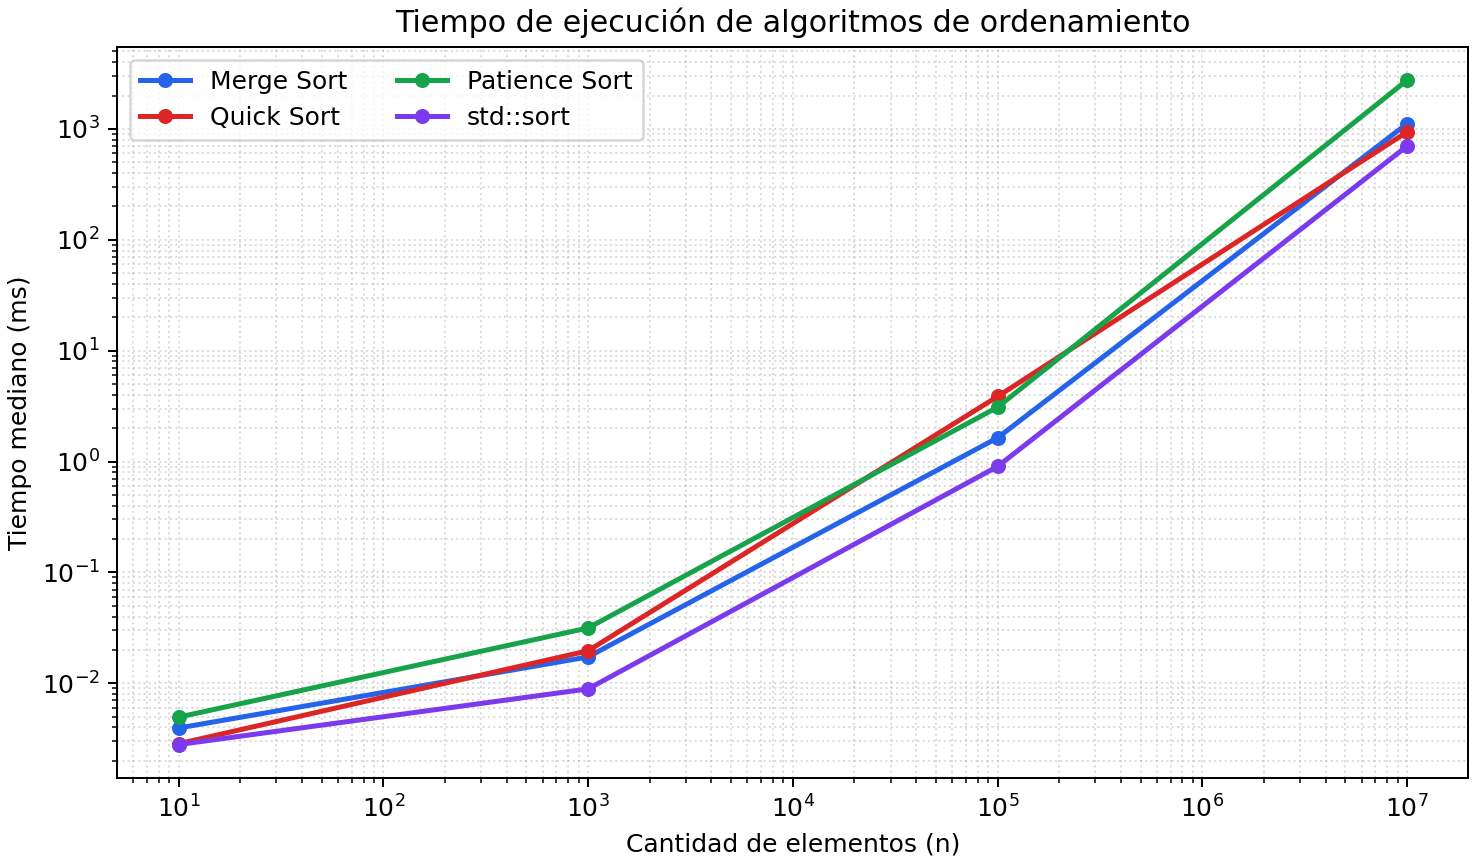
\includegraphics[width=0.49\textwidth]{../code/sorting/data/plots/sorting_time.png}}
    \hfill
    \subfloat[Memoria máxima.]{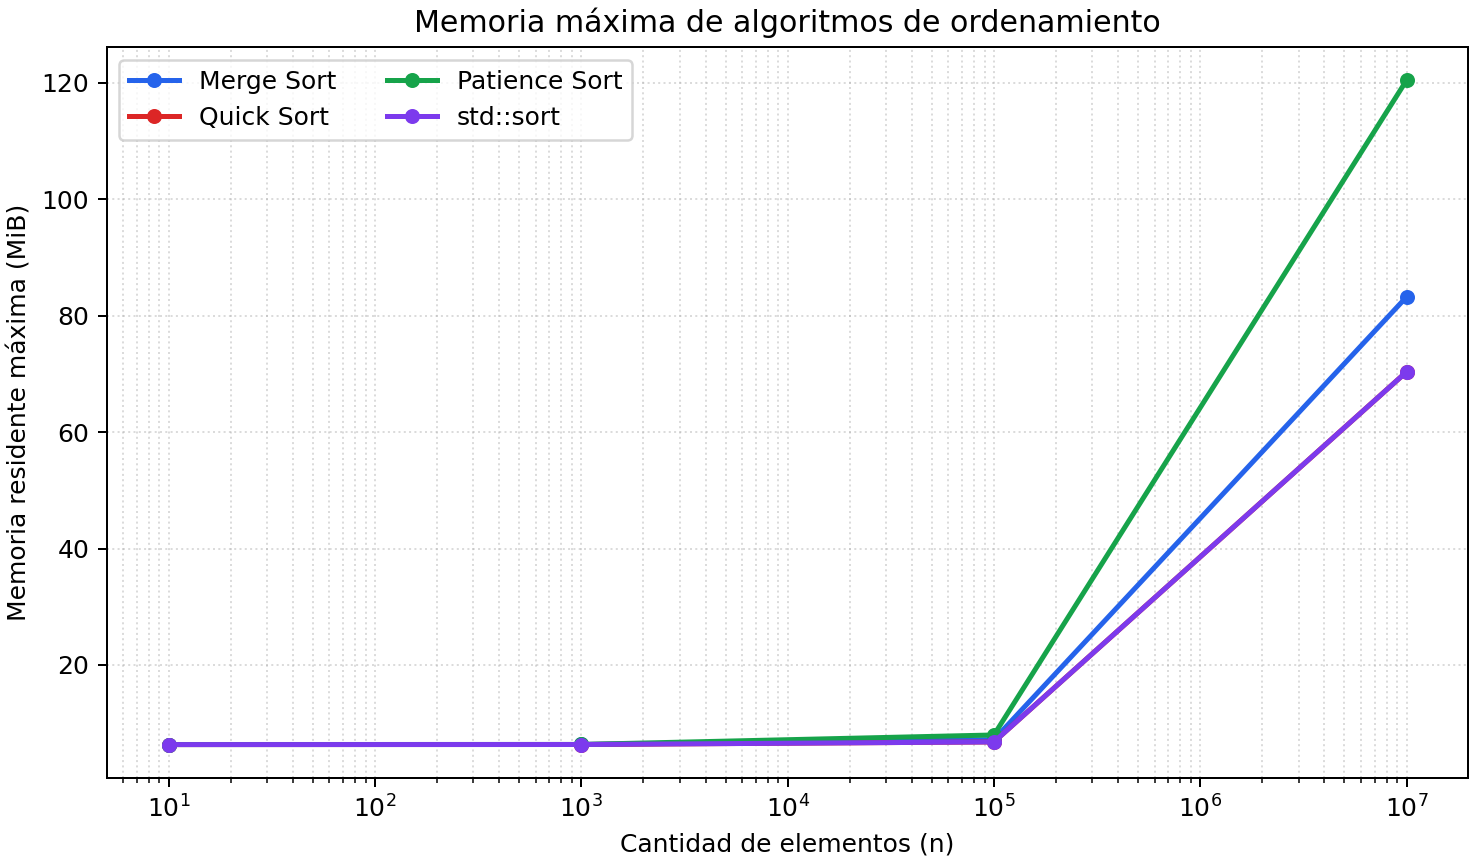
\includegraphics[width=0.49\textwidth]{../code/sorting/data/plots/sorting_memory.png}}
    \caption{Escalamiento de los algoritmos de ordenamiento. Los ejes de tiempo son logarítmicos.}
    \label{fig:sorting-scale}
\end{figure}

La distribución de entrada fue relevante (\cref{fig:sorting-distribution}).
Merge Sort detecta mitades ya ordenadas y por ello mejora en entradas
ascendentes. Patience Sort es especialmente rápido en orden descendente,
donde forma pocas pilas, y usa más memoria en orden ascendente. Quick Sort no
cae en el peor caso cuadrático gracias al pivote mediana de tres y la partición
ternaria, aunque su costo cambia con el dominio y la disposición de los
valores.

\begin{figure}[H]
    \centering
    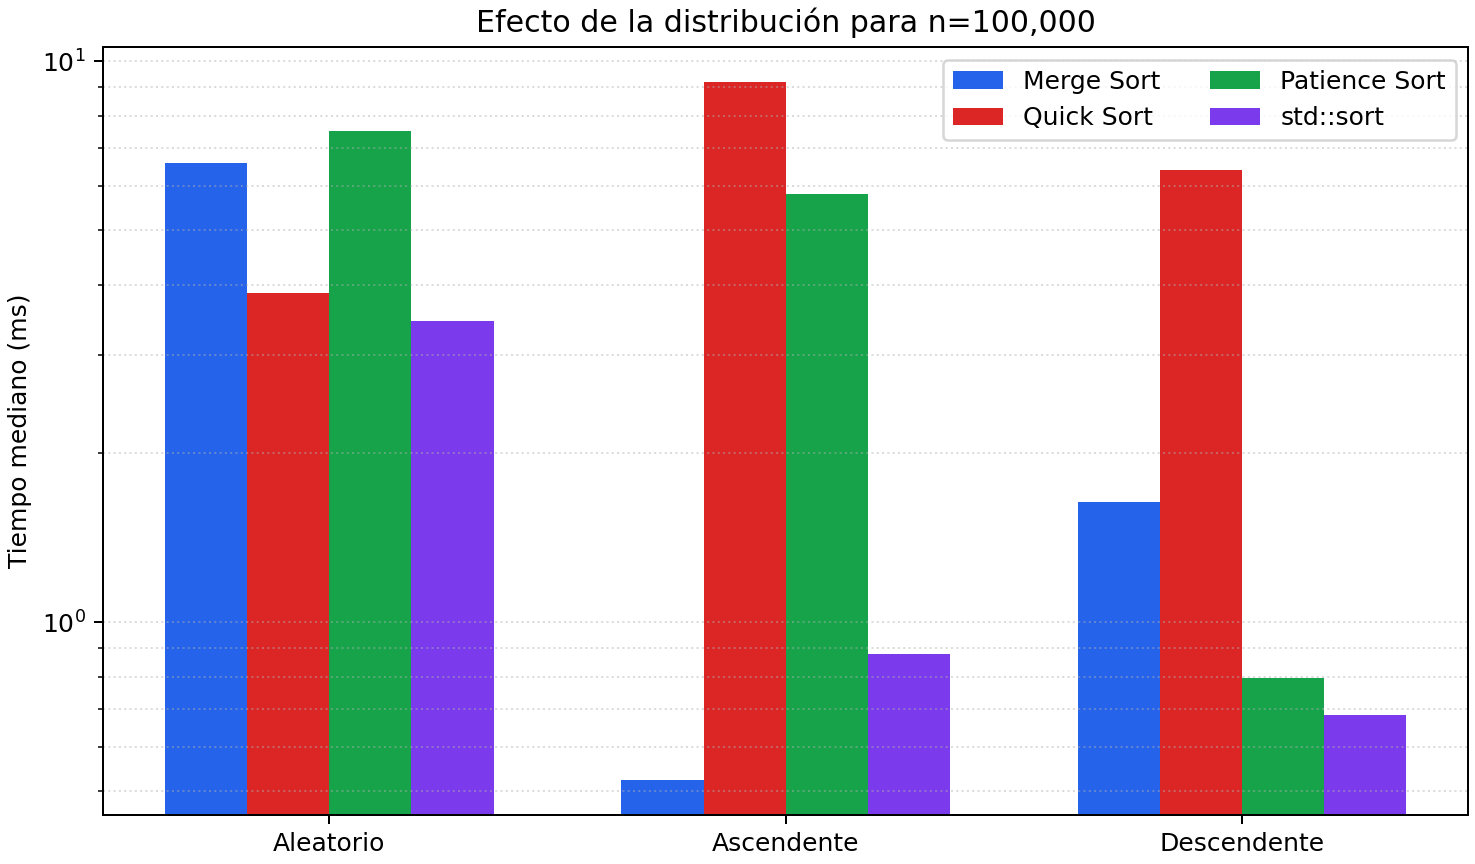
\includegraphics[width=0.78\textwidth]{../code/sorting/data/plots/sorting_by_distribution.png}
    \caption{Tiempo por distribución para $n=10^5$, agregado sobre dominios y muestras.}
    \label{fig:sorting-distribution}
\end{figure}

\subsection{Multiplicación de matrices}

El método naive tiene costo $O(n^3)$, mientras Strassen realiza siete
productos por nivel y alcanza $O(n^{\log_2 7})\approx O(n^{2.807})$
\cite{strassen1969}. En dimensiones pequeñas el caso base y la sobrecarga de
sumar y copiar submatrices dominan: para $n=256$, la mediana naive fue
\SI{9.497}{\milli\second} y Strassen \SI{12.763}{\milli\second}. En $n=1024$
se observó el cruce esperado: Strassen tardó \SI{668.944}{\milli\second}
frente a \SI{945.682}{\milli\second} del método naive, una reducción de
aproximadamente 29.3\%.

\begin{figure}[H]
    \centering
    \subfloat[Tiempo mediano.]{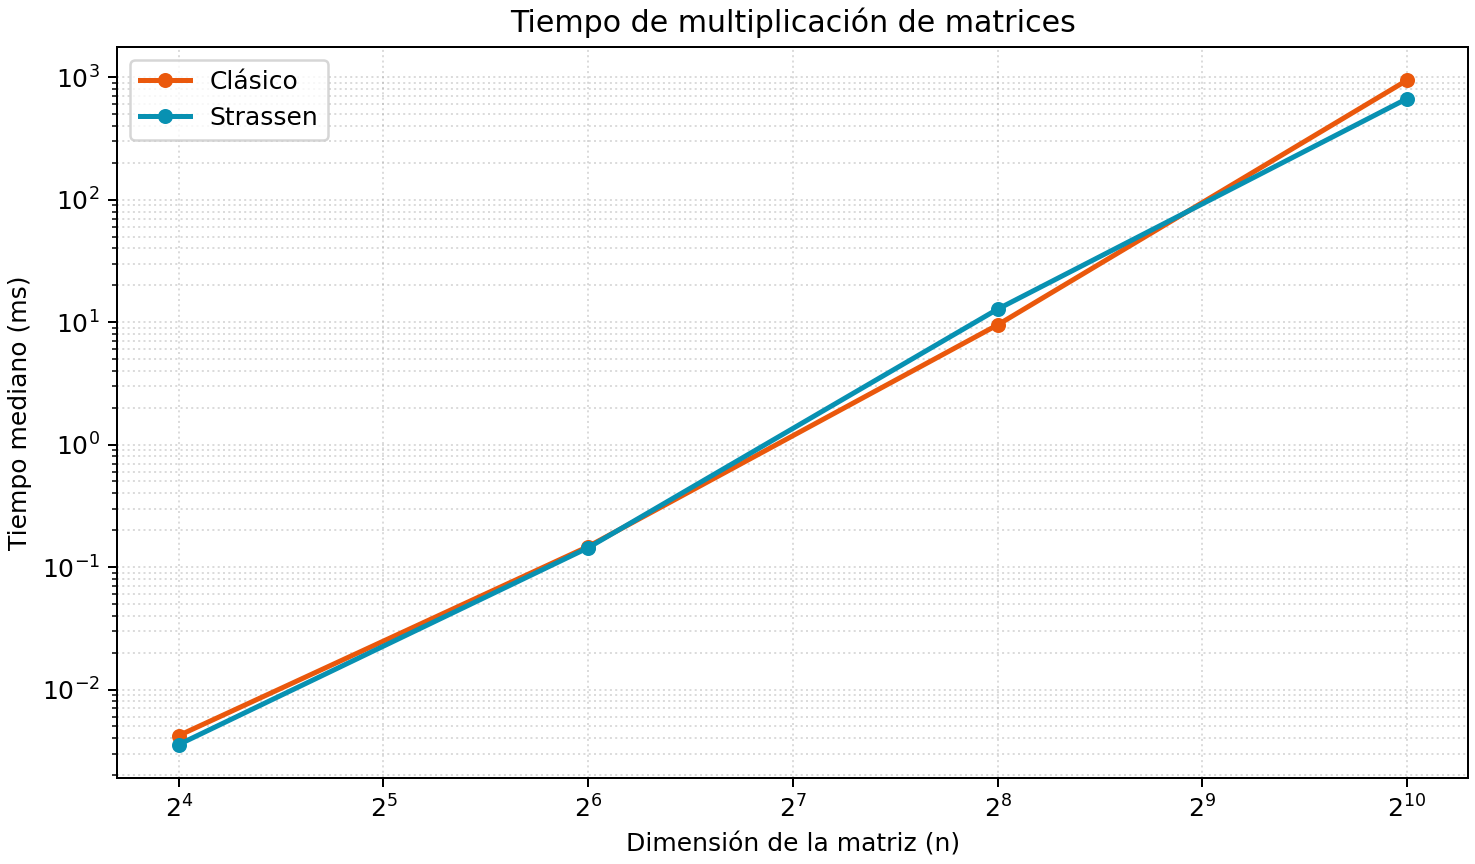
\includegraphics[width=0.49\textwidth]{../code/matrix_multiplication/data/plots/matrix_time.png}}
    \hfill
    \subfloat[Memoria máxima.]{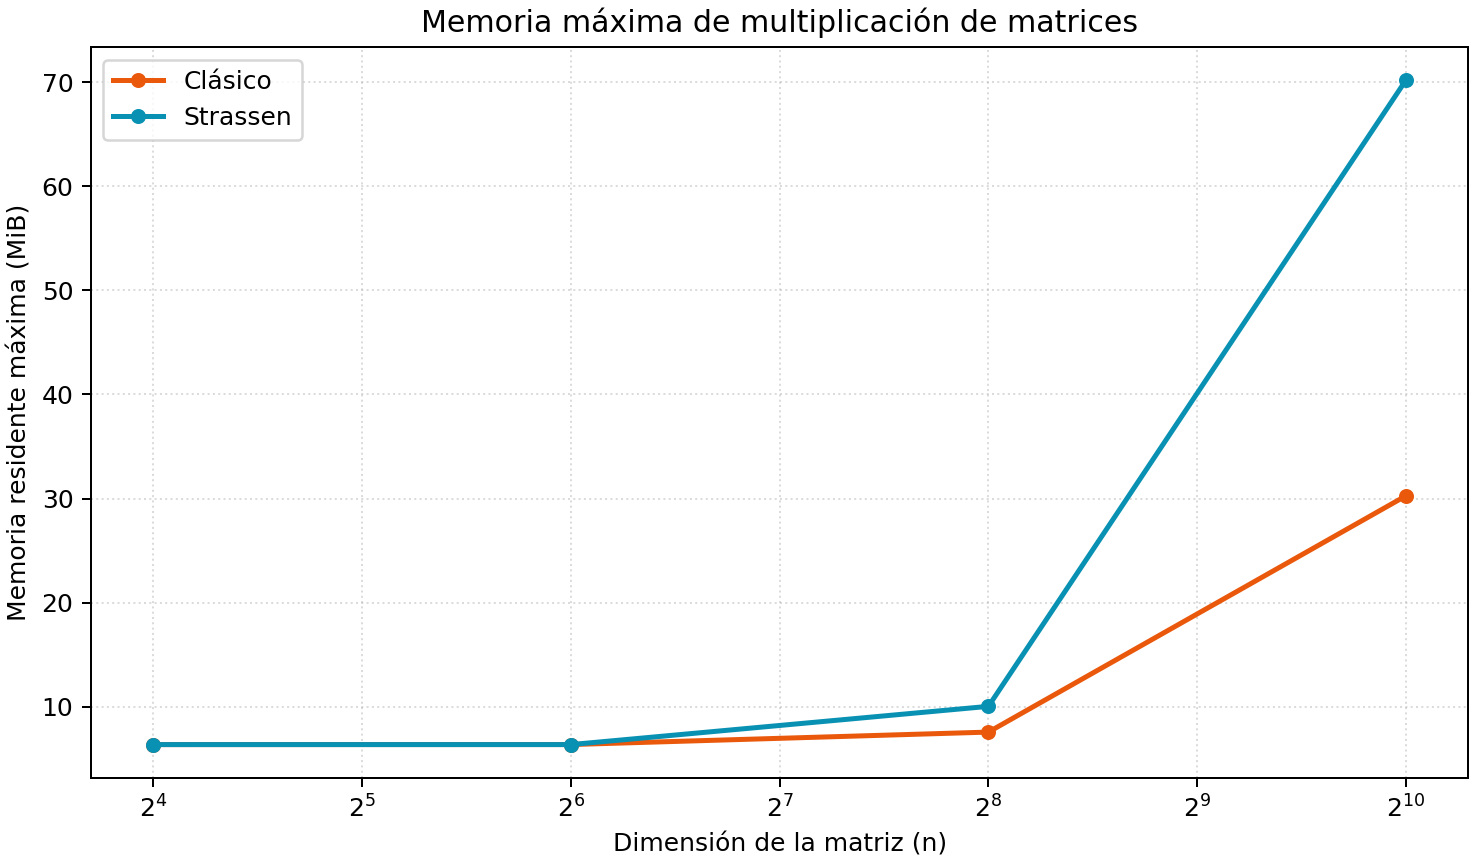
\includegraphics[width=0.49\textwidth]{../code/matrix_multiplication/data/plots/matrix_memory.png}}
    \caption{Escalamiento de la multiplicación de matrices.}
    \label{fig:matrix-scale}
\end{figure}

La ventaja temporal de Strassen tuvo un costo de memoria: en $n=1024$ usó
\SI{70.18}{\mebi\byte}, comparado con \SI{30.26}{\mebi\byte} del método
naive (\cref{fig:matrix-scale}). Como ambas implementaciones usan matrices
densas y no omiten ceros, el tipo disperso, diagonal o denso tuvo un efecto
menor que la dimensión. Los tiempos diminutos de $n=10$ y $n=16$ deben
interpretarse con cautela, pues son comparables al ruido del sistema; además,
los tamaños máximos tienen una sola muestra y no una mediana de 18 casos.
